\section{Current state of the application}
The current BI-DBS portal was deployed for the first time in 2016 \cite{bt-malec}. Over time it gained new features and grew large. Currently, it has a total of around 120000-140000 lines of code \cite{mt-plyskach}. Used technologies became less relevant and it became difficult to maintain it.

\subsection{Architecture}
The current application was built in a traditional way, using a monolithic architecture approach and following the Model-View-Presenter architectural pattern \cite{mvp-potel} \cite{architecture-haris}. Figure 1.1 shows the visualization of the architecture. The application is presented as one monolithic unit, and it is composed  of three components. 

\begin{itemize}
  \item \emph{The model:} Communicates with the database and handles domain and business logic.
  \item \emph{The view:} Provides visualization and directs user commands to the presenter, does not contain logic.
  \item \emph{The presenter:} Manages interactions between the database and the view. Receives data from the model and formats it to display in the view.
\end{itemize}

\begin{figure}[hp]
\centering
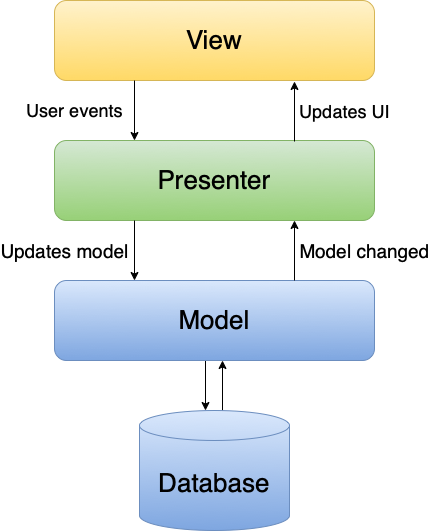
\includegraphics[scale=0.52]{../png/mvp_monolithic.png}
\caption{Monolithic architecture, MVP pattern}
\end{figure}

\noindent This architecture's main concept is having one code base that benefits in\newline simplifying development, testing, debugging, and deployment.\\
However, we can have those benefits only until the application grows large. Then all those processes get slower, more complex, and become problematic. In addition, with a lack of flexibility and scalability, it becomes challenging to maintain the application and keep it secure.\\

\noindent The BI-DBS portal is being developed by students. Students generally do not have much experience developing large applications and dealing with complex dependencies. Besides, they have limited time to progress in learning and then designing and developing the portal. Therefore it takes a lot of time for students to learn before contributing to the project. Thus it is more problematic for students to benefit from learning and for maintainers to keep it functioning correctly.


%%%%%%%%%%%%%%%%%%%%%%%%%%%%%%%%%%%%%%%%%%%%%%%%%%%%%%%%%%%%%%%%


\subsection{Technologies}
\paragraph*{PHP.} PHP is a general-purpose, open-source scripting language that can be integrated into HTML. \cite{php-doc,html-doc} It differs from client-side scripting languages in that its HTML is generated on a server and then sent to a client. That feature allows rapidly building a web application with a thick server and thin client. This is one of the approaches to using PHP to build an application, and it is used in the current project. \\
Using this approach leads to creating dependencies between the user interface and the application logic, which makes any changes more effortful since a developer needs to adjust it on both sides.

\paragraph*{Doctrine.} "Doctrine ORM is an object-relational mapper for PHP 7.1+ that provides transparent persistence for PHP objects. It sits on top of a powerful database abstraction layer. One of its key features is the option to write database queries in a proprietary object-oriented SQL dialect called Doctrine Query Language." \cite{doctrine-doc}\\ 
This framework did not cause problems during the development process and has no significant disadvantages for the correct operation of the BI-DBS.

\paragraph*{Nette.} Nette is an open-source framework for creating web applications in PHP. It helps with developing both the client and server sides of the application and also reduces security vulnerabilities. Moreover, it manages application states using sessions and routing. \cite{nette-doc}\\ 
Frontend and backend dependencies are strengthened, indicating that they are a single unit. The fact that they are so strongly dependent is a drawback. Because of this, it is difficult to make changes to one side without having an impact on the other. 

\paragraph*{Latte.} Nette framework uses a template system called Latte. It compiles templates down to the optimal PHP code. \cite{latte-doc}

\paragraph*{AdminLTE.} AdminLTE is a fully responsive administration template. Based on Bootstrap 4.6 framework and also the JS/jQuery plugin. \cite{adminlte-doc} 

\paragraph*{Vue 2.} Vue.js is a javascript framework for building user interfaces and single-page applications.\\
Most of the frontend is implemented using Latte templates and AdminLTE bootstrap. However, in order to reduce dependencies between the frontend and the backend and also modernize it, a few components were refactored to the Vue.js version 2. The logic is defined using the Options API. It is a traditional object-oriented way, and up until Vue 2 it was the only way to create components in Vue. \cite{vue2-doc, apivue-dzakelsek}

\paragraph*{Javascript.} JavaScript is a high-level programming language used for defining the behavior of webpages. It is a dynamically-typed scripting language that lets you control multimedia, animate graphics, and generate dynamically changing content. \cite{js-doc}\\ 
In the current BI-DBS portal it is used for defining logic on the frontend. Dynamically-typed languages are easy for development, but this feature reduces the code's readability, requires more testing and are prone to run-time errors. Large applications like BI-DBS are likely to experience problems as a result of its drawbacks because it is better suited for smaller applications with simple logic.

\paragraph*{Webpack.} Primarily, Webpack is a static module bundler for modern JavaScript programs. When Webpack processes your application, it internally creates a dependency tree from one or more entry points and then merges every module your project requires into one or more bundles. \cite{webpack-doc}\\
Webpack is used in a current application for bundling a few modernized frontend components implemented in Vue.js and javascript.

%%%%%%%%%%%%%%%%%%%%%%%%%%%%%%%%%%%%%%%%%%%%%%%%%%%%%%%%%%%%%%%%